\documentclass[11pt]{beamer}
\usepackage[utf8]{vietnam}
\usepackage{lmodern}
\usetheme{Warsaw}
\usepackage[backend=biber]{biblatex}

\addbibresource{presentation.bib}

\newcommand{\eg}{\text{e.g.\ }}

\begin{document}
\author{Trần Hoàng Quân, Lê Hoàng Trọng Tín, Lê Mai Nguyên Thảo}
\title{Trust Negotiations}
\subtitle{Tìm hiểu khái niệm và một số hệ thống thực tế}
\logo{
\includegraphics[scale=.2]{img/fithcmuslogo.png}}
\institute{Trường Đại học Khoa học tự nhiên - ĐHQG HCM \\ Khoa Công nghệ Thông tin}
%\date{}
%\setbeamercovered{transparent}
%\setbeamertemplate{navigation symbols}{}
\begin{frame}[plain]
\maketitle
\end{frame}

\begin{frame}
\frametitle{Nội dung}
\tableofcontents
\end{frame}

\section{Giới thiệu}
\begin{frame}{Giới thiệu}
Một ví dụ trong thế giới thực: Bạn đi siêu thị mua hàng và thanh toán bằng thẻ tín dụng.
\begin{enumerate}
\item Nhân viên thu ngân xác nhận thẻ của bạn hợp lệ (\eg kiểm tra format số thẻ, kiểm tra 4 số security code, kiểm tra thẻ có bị chỉnh sửa tẩy xóa, ..etc).
\item Nhân viên thu ngân yêu cầu chủ thẻ nhập PIN và nhập số tiền.
\item Nhân viên thu ngân in biên lai và đưa bạn kí.
\item Nhân viên xác nhận chữ kí của bạn giống chữ kí phía sau thẻ, vậy là đã thanh toán thành công.
\end{enumerate}
\end{frame}

\begin{frame}{Giới thiệu (cont.)}
Giao dịch trong ví dụ trên có sự trao đổi thông tin (credentials) giữa người mua và người bán, từ đó thiết lập sự tin tưởng rằng người mua có đủ điều kiện để mua đồ, và người bán có đủ điều kiện để bán.

Mục đích cuối cùng của Trust Negotiation:
\begin{itemize}
\item Thiết lập sự tin cậy (Trust Establishment) giữa các bên tham gia.
\item Dù trao đổi nhiều thông tin (credentials) với nhau, credentials phải được giữ an toàn.
\end{itemize}
\end{frame}

\section{Trust Negotiation}
\begin{frame}{Trust Establishment}
Trust Establishment: thiết lập sự tin cậy giữa những "người lạ" trong hệ thống mở:
\begin{itemize}
\item Client và Server không cùng security domain.
\item Quyết định cấp quyền truy cập dựa vào thuộc tính (attribute), không dựa vào danh tính (identity).
\begin{itemize}
\item \eg Quyền của client trong tổ chức, loại ngành nghề, chức vụ, ..etc
\end{itemize}
\end{itemize}
\end{frame}

\begin{frame}{Trust Negotiation}
Trust Negotiation: phuơng pháp tiếp cận bằng cách kiểm soát truy cập (access control) và xác thực (authentication), cho phép người yêu cầu tài nguyên (resource requesters) và nhà cung cấp (providers) thiết lập sự tin cậy trong các hệ thống mở, dựa trên các thuộc tính (attributes) hơn là danh tính (identity).
\begin{itemize}
\item Trao đổi digital credentials giữa các bên một cách tuần tự.
\item Đầu tiên trao đổi credentials ít nhạy cảm, khi độ tin cậy tăng thì trao đổi credentials nhạy cảm hơn.
\end{itemize}
\end{frame}


\begin{frame}{Trust Negotiation (cont.)}
\begin{figure}[H]
\centering
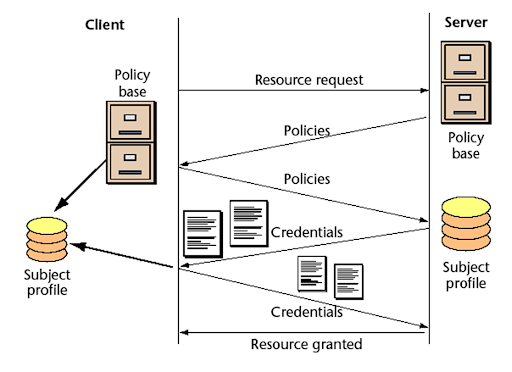
\includegraphics[scale=.4]{img/trust-simple.png}
\caption{Sơ đồ (đơn giản) của một mô hình Trust Negotiation}
\end{figure}
\end{frame}

\begin{frame}{Trust Negotiation (cont.) - Digital Credentials}
Digital Credentials: chứa các thuộc tính thông tin của người sở hữu, được cấp bởi một bên đáng tin cậy (thường là nhà cung cấp chứng thư số).
\begin{itemize}
\item Khó làm giả.
\item Dễ xác thực.
\item Ký bằng PKI (public-key infrastructure, \eg chuẩn X.509 v3)
\end{itemize}
\end{frame}

\begin{frame}{Trust Negotiation (cont.) - Credential disclosure}
Credential disclosure policy (CDP):
\begin{itemize}
\item Điều kiện để một bên công bố các tài nguyên.
\item Bản thân credentials có thể có một số thông tin nhạy cảm, nên cũng được xem là một tài nguyên được bảo vệ.
\item Bản thân CDP cũng là một đối tượng được bảo vệ.
\end{itemize}
\end{frame}

\begin{frame}{Trust Negotiation (cont.) - Requirements}
Các yếu tố cần thiết cho một hệ thống Trust Management:
\begin{itemize}
\item Quyền sở hữu đối với credential.
\item Tính hợp lệ của credential.
\item Cơ chế bảo vệ quyền riêng tư.
\item Hỗ trợ các chiến thuật thương lượng thay thế.
\item Các chiến thuật thương lượng nhanh.
\end{itemize}
\end{frame}

\begin{frame}{Trust Negotiation (cont.)}
Một số hệ thống trên thực tế:
\begin{itemize}
\item Keynote trust management system
\item Trust Establishment phát triển bởi Haifa Research lab
\begin{itemize}
\item Trust Policy Language (TPL)\cite{848442}
\end{itemize}
\item TrustBuilder
\item Unipro
\item Trust-X
\end{itemize}
\end{frame}

\section{Một số hệ thống trên thực tế}
\subsection{ATNAC}
\begin{frame}{ATNAC}
Adaptive Trust Negotiation and Access Control (ATNAC)\cite{10.1145/1063979.1064004} là kiến trúc access control cho các dịch vụ điện tử, kết hợp của hai hệ thống:
\begin{itemize}
\item TrustBuilder: Xác định cách thức tiết lộ thông tin nhạy cảm.
\item GAA-API: Kiểm soát truy cập một cách thích ứng.
\end{itemize}
\end{frame}

\begin{frame}{ATNAC (cont.) - Trust Builder}
TrustBuilder là hệ thống Trust Negotiation phát triển bởi Đại học Brigham Young (BYU) và Đại học Illinois Urbana-Champaign (UIUC):
\begin{itemize}
\item Dễ bị tấn công DoS (denial of service - từ chối dịch vụ).
\begin{itemize}
\item Số lượng lớn session Trust Negotiation được gởi lên server.
\item Server phải tính toán policy rất phức tạp.
\item Server phải tính toán credentials không liên quan hoặc không hợp lệ.
\end{itemize}
\item Các cuộc tấn công thường nhắm vào thông tin nhạy cảm.
\end{itemize}
\end{frame}

\begin{frame}{ATNAC (cont.) - GAA-API}
GAA-API: Generic Authorization and Access-control API
\begin{itemize}
\item Là middleware API
\item Fine-grained access control (FGAC - Kiểm soát truy cập chi tiết).
\item Phát hiện và phản hồi xâm nhập cấp ứng dụng.
\item Có thể tương tác với hệ thống phát hiện xâm nhập (Intrusion Detection System - IDS) để thích ứng với các điều kiện đe dọa mạng.
\item Không hỗ trợ Trust Negotiation.
\end{itemize}
\end{frame}

\begin{frame}{ATNAC (cont.) - GAA-API}
\begin{figure}
    \centering
    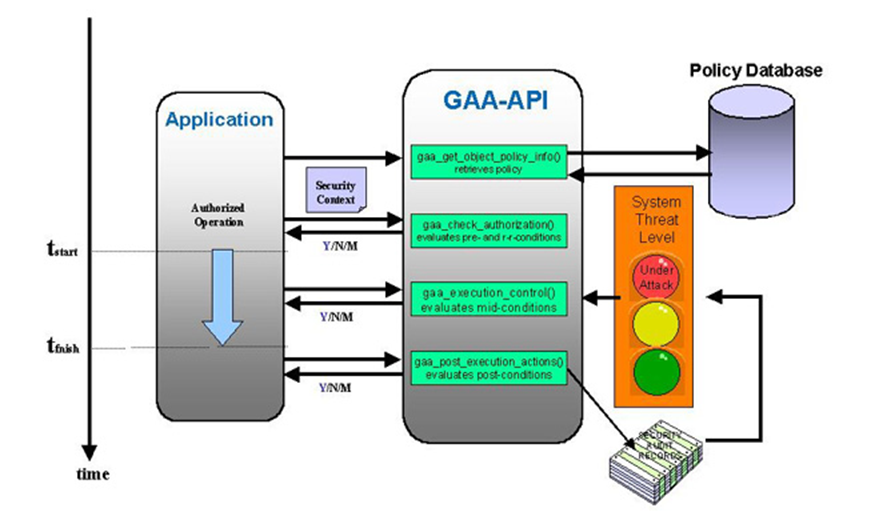
\includegraphics[scale=.5]{img/gaa-api.png}
    \caption{Sơ đồ hệ thống với GAA-API middleware}
    \label{fig:gaa_api}
\end{figure}
\end{frame}

\begin{frame}{ATNAC (cont.)}
Đặc điểm của ATNAC:
\begin{itemize}
\item Kết hợp hệ thống access control và Trust Negotiation để vá  khuyết điểm của mỗi hệ thống.
\item Hỗ trợ các chính sách thích ứng chi tiết (Fine-grained adaptive policies).
\item Giảm chi phí tính toán.
\end{itemize}
\end{frame}

\begin{frame}{ATNAC (cont.)}
Chức năng từng phần của ATNAC:
\begin{itemize}
\item GAA-API:
\begin{itemize}
\item Quy định access control policies cho tài nguyên, dịch vụ và hành động.
\item Các policies được thể hiện theo format EACL (Enhanced Access Control List).
\end{itemize}
\item TrustBuilder:
\begin{itemize}
\item Thi hành các policies bảo vệ thông tin nhạy cảm.
\item Dùng chứng chỉ số X.509 v3.
\item Dùng TPL policies.
\end{itemize}
\end{itemize}
\end{frame}

\begin{frame}{ATNAC (cont.) - framework}
\begin{figure}
\centering
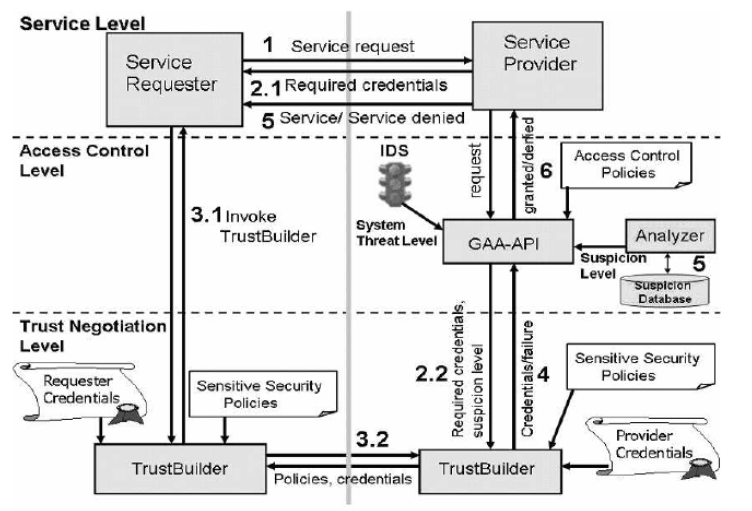
\includegraphics[scale=.5]{img/atnac.png}
\caption{Sơ đồ ATNAC framework}
\label{fig:atnac}
\end{figure}
\end{frame}

\begin{frame}{ATNAC (cont.) - Suspicion Level}
Mức nghi ngờ (Suspicion level) đánh giá khả năng một requester đang thực hiện hành động không phù hợp. Mỗi requester của một service có một Suspicion Level riêng biệt. Gồm 3 thành phần chính:
\begin{itemize}
\item $S_\text{DOS}$: Khả năng requester đang thực hiện tấn công DoS.
\item $S_\text{IL}$: Rò rỉ thông tin (information leakage).
\item $S_\text{O}$: Các hành vi còn lại.
\end{itemize}
Suspicion Level tăng khi một sự kiện đáng nghi xảy ra, giảm khi một sự kiện (được cho là) tích cực xảy ra.
\end{frame}

\begin{frame}{ATNAC (cont.) - Cách hoạt động}
\begin{itemize}
\item Analyzer xác định các requesters gởi một số lượng request tương đồng cao bất thường và tăng $S_\text{DOS}$.
\item Trong quá trình trust negotiation, credentials gởi bởi client phải trùng với credentials hệ thống yêu cầu, nếu không $S_\text{DOS} = 1$.
\item Nếu $S_\text{DOS}, S_\text{IL}$ hoặc $S_\text{O} > 0.9$, hệ thống sẽ dùng firewall chặn requester.
\item Nếu $S_\text{IL} > \textit{một ngưỡng nhất định}$, TrustBuilder sẽ áp các chính sách nghiêm ngặt hơn với credentials, nhất là các credentials nhạy cảm.
\item Khi $S_\text{IL}$ tăng, GAA-API dùng các access control policies chặt chẽ hơn.
\end{itemize}
\end{frame}

\begin{frame}{ATNAC (cont.) - ví dụ}
\begin{columns}
\begin{column}{0.5\textwidth}
\begin{figure}
    \centering
    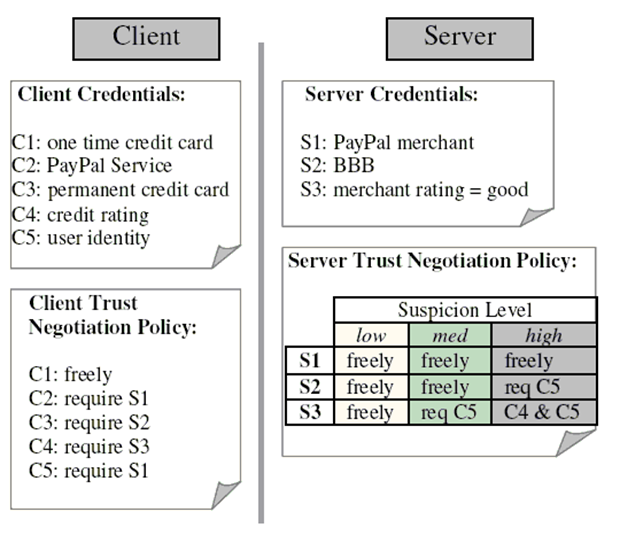
\includegraphics[scale=.4]{img/atnac-example-1.png}
    \caption{Credentials và Policies của client và server}
    \label{fig:atnac-1}
\end{figure}
\end{column}
\begin{column}{0.5\textwidth}
\begin{figure}
    \centering
    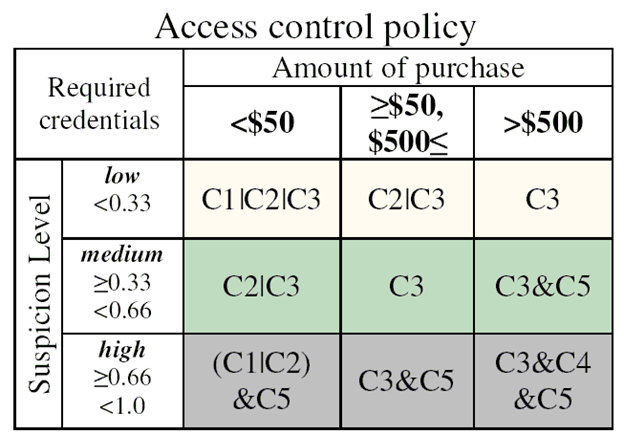
\includegraphics[scale=.4]{img/atnac-example-2.png}
    \caption{Access control policy}
    \label{fig:atnac-2}
\end{figure}
\end{column}
\end{columns}
\end{frame}

\subsection{Trust-X}
\begin{frame}{Trust-X}
Trust-X: P2P framework dành cho Trust Establishment\cite{10.1109/TKDE.2004.1318565}
\begin{itemize}
\item Hệ thống dựa trên XML
\item Thiết kế cho môi trường P2P.
\begin{itemize}
\item Mỗi bên chịu trách nhiệm tương đương trong quản lý thương lượng (negotiation management).
\item Bên nào cũng có thể là requester hoặc controller của một resource.
\end{itemize}
\item X-TNL: Ngôn ngữ đặc tả các chứng chỉ và policies dựa trên nền XML.
\end{itemize}
\end{frame}

\begin{frame}{Trust-X (cont.)}
\begin{itemize}
\item Chứng chỉ: có 2 loại:
\begin{itemize}
\item Credentials: Thể hiện đặc điểm của chủ sở hữu, được công nhận bởi CA (certificate authority).
\item Declarations: Chứa thông tin của chủ sở hữu, không cần được chứng nhận.
\end{itemize}
\item Trust tickets (X-TNL): dùng để tăng tốc quá trình negotiation khi đã được cấp quyền truy cập trong lần negotiation trước.
\item Negotiation tiến hành theo từng giai đoạn.
\end{itemize}
\end{frame}

\begin{frame}{Trust-X (cont.) - Kiến trúc}
\begin{figure}
\centering
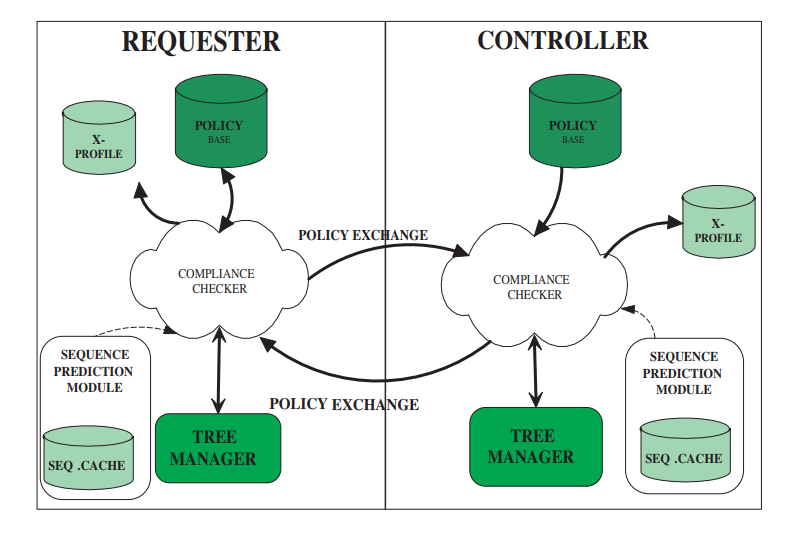
\includegraphics[scale=.5]{img/trust-x-architecture.PNG}
\caption{Kiến trúc mô hình Trust-X}
\label{fig:trust_x_architecture}
\end{figure}
\end{frame}

\begin{frame}[allowframebreaks]{Tài liệu}
\printbibliography
\end{frame}
\end{document}